\section{Introduction} \label{sec:ch4_estimateurs_robustes}
On détaille ici le domaine des \og statistiques robustes\fg{}, dénommées ainsi d'après le livre de Hubert (\cite{Huber1981}). On cherche dans ce domaine à définir des estimateurs robustes, dans le sens où l'estimation produite à partir d'échantillons n'est pas modifiée significativement si une ou plusieurs valeurs sont évidemment marginales par rapport à un ensemble de référence. Il ne s'agit pas d'un domaine intrinsèquement lié à l'odométrie visuelle ou à la reconstruction de l'environnement, mais les techniques qui y sont développées peuvent être exploitées dans ces cas de figure.\\

On ne considère pas ici une densité de probabilité gaussienne pour les échantillons, celle-ci étant parfaitement mesurée par les opérateurs courants de moyenne géométrique et de variance. Comme nous avons déjà eu l'occasion de l'expliquer, différents phénomènes peuvent éloigner significativement les mesures de cette distribution dans certains problèmes. Ce domaine des statistiques n'est pas à proprement parler intrinsèque aux étapes d'estimation de l'ego-motion et de reconstruction de l'environnement. Il est cependant présent dans la littérature de ce domaine (par exemple \cite{Zou}), et nous proposons de l'utiliser dans notre approche. Nous en détaillons donc les motivations et quelques uns des enseignements dans cette brève introduction technique.

\section{Définitions}
On définit tout d'abord quelques métriques nous permettant ensuite d'illustrer les avantages d'une approche robuste des statistiques.

\subsection{Variance:}
Il s'agit d'une mesure de la fonction de distribution d'une variable aléatoire, qui correspond à son second moment statistique. Elle se définit en général pour une variable discrète par (avec $E$ l'espérance et $\mu = E(X)$) :
\begin{equation}
Var(X) = E((X-\mu)^2)
\end{equation}
On ne prend pas en compte d'éléments fautifs dans cette définition, c'est-à-dire que toutes les observations correspondent bien à la variable $X$. Dans le cas d'observations polluées par du bruit, d'autres estimateurs convergeant vers la variance de la distribution visée sont possibles et parfois souhaitables (cf. section \ref{sec:ch4_exemples_statitistiques}).

\subsection{Point de rupture:}
Cette quantité est définie comme étant le pourcentage de points marginaux acceptés par un estimateur avant de voir sa valeur altérée. En notant $\Sigma$ un estimateur, on peut noter la définition du point de rupture (\emph{Breakdown Point}) comme étant : \\
\begin{equation}
BP_{\Sigma} = \min(\frac{N_{Outliers}}{N_{Inliers}}) \; | \; \{\Sigma (Inliers) \neq \Sigma(Inliers\, + \,Outliers) \} 
\end{equation}

\subsection{Efficacité:}
On peut par ailleurs définir l'efficacité relative d'un estimateur $\tilde{\theta}$ par rapport à l'estimateur $\hat{\theta}$ par le rapport inversé de leurs variances :
\begin{equation} \label{eq:ch4_ARE}
RE \left( \tilde{\theta}, \hat{\theta}\right)  = \frac{var(\hat{\theta})} {var(\tilde{\theta})}
\end{equation}
Ce ratio n'a de sens que si les estimateurs en question ne sont pas biaisés, dans le sens où leur variance n'est pas inférieure à la variance réelle des échantillons. Il est possible dans ce cas d'estimer ce biais, ou encore de définir une efficacité invariante (par exemple en utilisant la variance du logarithme de l'estimation). On note ARE (\emph{Asymptotic Relative Efficiency}, Efficacité Relative Asymptotique) la limite de RE quand le nombre d'échantillons tend vers $\infty$. Cette mesure est souvent utilisée pour comparer un estimateur optimal pour une distribution Gaussienne à un estimateur dont la convergence est plus lente, mais plus résistante au bruit.

\subsection{Robustesse:}
La définition proposée par Huber (\cite{Huber1981}) pour quantifier la robustesse d'un estimateur est liée à une notion de continuité des valeurs estimées. Elle s'écrit formellement (en reprenant les notations de Huber), avec $(T_n)$ la séquence d'estimations, $F$ la fonction de distribution des échantillons, $F_0$ une fonction de distribution de référence (par exemple gaussienne), et $d$ une métrique sur l'espace des distributions considéré : 
\begin{align}
	\begin{split}
		T_n \:& \textnormal{robuste en F} = F_0 \Leftrightarrow \\
		& \forall \epsilon > 0, \:  \exists (\delta, n_0) > 0 \: | \\
		& \qquad	\forall F \:  et \:  \forall n \geq n_0 : \\
		& \qquad \qquad	d(F,F_0) \leq \delta \Rightarrow d(L_{F_0}(T_n), L_{F}(T_n)) \leq \epsilon
	\end{split}
\end{align}

\section{Quelques exemples}
\subsection{Calculs de variance, efficacité variable:}\label{sec:ch4_exemples_statitistiques}
La comparaison de la médiane et de la moyenne, estimateurs couramment utilisés du centre d'une fonction de distribution, est intéressante lorsqu'appliquée à ces différentes métriques à partir d'une distribution gaussienne : la moyenne est beaucoup plus "<efficace"> que la médiane (ARE(mediane, moyenne) = 0.64), mais l'ajout de points marginaux (par exemple issus d'une autre distribution gaussienne) l'affecte beaucoup plus rapidement. On peut facilement s'en convaincre, la valeur de la moyenne étant modifiée dès l'altération d'un unique échantillon. La médiane est en ce sens plus robuste, la moitié des échantillons devant être modifiés avant de changer la valeur de cet estimateur (si l'on suppose une altération aléatoire et uniforme). \\
L'estimation de la "<largeur"> d'une distribution est l'objet d'un autre exemple de Tukey (\cite{Tukey1960}), que nous reprenons ici, illustrant quantitativement ce phénomène. Cet exemple est également repris dans les notes de cours de B. Ripley (\cite{Ripley2004}), dont nous reprenons les calculs. Considérons $n$ observations $Y_i$ tirées d'une fonction de distribution donnée. Supposons tout d'abord que cette fonction de distribution soit une loi normale, de moyenne $\mu$ et de variance $\sigma^2$ (notée $N(\mu, \sigma)$). On considère les estimateurs $\hat{\sigma}$ et $\tilde{\sigma}$ tels que:
\begin{align}
	\begin{split}
		\hat{\sigma}^2 &= s^2 = \frac{1}{n} \sum\limits_{i=1}^{N} (Y_i - \mu)^2 \\
		\tilde{\sigma}^2 &= d^2 \cdot \frac{\pi}{2}
	\end{split}
\end{align}
avec $\bar{Y}$ le centre de masse des points $Y_i$ et 
\begin{equation*}
	d = \frac{1}{n} \sum\limits_{i=1}^{N} \left| Y_i - \bar{Y}\right| 
\end{equation*}
La normalisation de $\tilde{\sigma}^2$ est choisie pour que ces opérateurs soient égaux pour une distribution normale. Leur efficacité relative (pour un nombre d'échantillons tendant vers $\inf$ en reprenant \ref{eq:ch4_ARE}) vaut : $ARE(\hat{\sigma}^2, \tilde{\sigma}^2) = 0.88$. On peut montrer que $\hat{\sigma}$ est effectivement l'estimateur optimal pour la loi normale.\\

On propose, pour rendre compte d'une source de bruit indépendante, de générer une séquence de points tels que chaque point a une probabilité $1- \epsilon$ d'être selon la loi normale $N(\mu, \sigma)$ et une probabilité $\epsilon$ d'être selon la loi normale $N(\mu, 9\sigma)$. L'évolution de l'efficacité relative de nos deux estimateurs en fonction de $\epsilon$ est visible sur le tableau \ref{tab:ch4_robust_stat_mix}. 

\begin{figure}
	\begin{equation*}
		\begin{tabular} {| c | c |}
			\hline
			$\epsilon ( \%)$ & $ARE(\hat{\sigma}^2, \tilde{\sigma}^2) $\\
			\hline
			0 	& 0.88 	\\
			0.1 & 0.95 	\\
			0.2 & 1.0 	\\
			1 	& 1.4 	\\
			5 	& 2.0		\\
			\hline
		\end{tabular}
	\end{equation*}
	\caption{Efficacité relative des estimateurs $\hat{\sigma}$ et $\tilde{\sigma}$ en fonction de $\epsilon$}
	\label{tab:ch4_robust_stat_mix}
\end{figure}

La variance de ces observations reste proportionnelle à $\sigma^2$, et notre métrique est invariante d'échelle. On constate aisément que l'avantage en efficacité du calcul de la variance "classique" est très vite remis en cause en présence de bruit, 0.2\% de points faux étant suffisants en pratique pour que le calcul basé sur la somme des écarts absolus soit plus efficace. D'autres opérateurs sont possibles pour estimer la variance de la distribution, celui présenté dans cet exemple étant mis en avant pour illustrer les différences de comportement possibles en présence de bruit. Les deux opérateurs présents ont notamment un point de rupture de 0\%, ce qui est en général préjudiciable, et peut être mitigé par d'autres opérateurs basés par exemple sur l'usage d'une médiane. On pourra notamment introduire l'opérateur MAD (\emph{Median of Absolute Differences}, Médiane des écarts à la médiane), qui est utilisé dans notre implémentation :
\begin{equation} \label{eq:ch4_MAD}
MAD = \frac{1}{0.6745} médiane_{i \in [i,N]} { \left| Y_i - médiane_{j \in [j,N]}(Y_j) \right\|}
\end{equation}
Cet opérateur n'est pas très efficace\footnote{Au sens de l'ARE, celle ci étant de 0.37 si on le compare à $\hat{\sigma}$ pour une loi normale.}, mais très robuste aux points aberrants. Le coefficient de 0.6745 fait office de normalisation, rendant l'opérateur MAD exactement égal à $\hat{\sigma}$ dans le cas de la loi normale.

\subsection{Régression relative à un modèle - algorithme RANSAC:}
Une des stratégies les plus utilisées de nos jours pour estimer les paramètres d'un modèle au sein de mesures bruitées a recours à une recherche aléatoire de consensus. Connue sous le nom de Ransac (\emph{RAndom SAmple Consensus}), elle fut proposée par Fischler et Bolles \cite{Fischler1981}. Cette méthode a besoin d'un modèle, par exemple une surface paramétrique ou un mouvement, permettant d'évaluer le statut des échantillons comme marginaux ou non. Partant de ce modèle, il s'agit ensuite de réaliser des tirages aléatoires parmi l'ensemble de valeurs disponibles, de calculer les paramètres du modèle approchant le plus la distribution, et de compter finalement le nombre d'échantillons en accord avec ce modèle. Le tirage aléatoire conduisant au plus grand nombre de points en accord avec le modèle est retenu, justifiant l'appellation de recherche aléatoire de consensus.\\

En fonction des paramètres de convergence choisis (notamment du seuil conduisant à l'appartenance d'un échantillon au modèle), on peut obtenir avec cet estimateur un point de rupture très grand, bien au delà des 50\%, dans le cas d'un bruit aléatoire de moyenne nulle. Il s'agit cependant d'un estimateur particulier, nécessitant une connaissance \emph{a priori} du résultat attendu, sous la forme d'un modèle paramétrique. Par ailleurs, il suppose qu'il existe une limite déterminée permettant d'isoler de manière arbitraire les points marginaux des points cohérents, ce qui n'est pas nécessairement le cas. Il est par exemple difficile de mettre en œuvre un tel algorithme dans le cas d'estimation de variables multimodales, dans lequel le modèle et les critères d'appartenance des points à une distribution principale sont délicats à déterminer.

\subsection{M-estimateurs:}
Si l'on considère le problème de l'estimation de la valeur centrale d'une fonction de densité de probabilité, plusieurs estimateurs sont couramment utilisés. On pourra citer la moyenne et la médiane bien sûr, mais aussi la moyenne tronquée (on néglige les "<ailes"> de la fonction de distribution, par le biais d'un coefficient $\alpha$ qui désigne la fraction des points extrêmes - les plus éloignés de la moyenne - à négliger). Il est cependant courant d'utiliser les \textit{M-estimateurs}, estimateurs basés sur le calcul du maximum (d'où le M) de vraisemblance. Cette vraisemblance est déterminée par rapport à la fonction de densité de probabilité modèle $f$, et on introduit souvent la fonction $\rho = -log(f)$ qui simplifie les calculs. L'estimateur maximisant la vraisemblance conduit à minimiser $\rho$, en supposant que les échantillons soient indépendants:

\begin{equation}
\min_{\mu} \sum\limits_{i}^{n} -log f(Y_i - \mu) = \min_{\mu} \sum\limits_{i} \rho(Y_i - \mu)
\end{equation}

La fonction de densité de probabilité doit cependant être connue pour maximiser la vraisemblance et obtenir un estimateur, et celle-ci n'est pas nécessairement déterminée de manière exacte. Cette formule est par ailleurs exacte pour un grand nombre d'échantillons, mais n'assure pas nécessairement une convergence rapide de l'estimateur. Il est possible, comme le propose Huber \cite{Huber1981} de choisir une fonction $\rho = log(f)$ arbitraire dont on minimise la somme des contributions sur les échantillons. 
\begin{equation}
\hat{\mu}_{ML} = \arg\min_\mu \sum\limits_{i}^{n} \rho(Y_i, \mu)
\end{equation}
Avec cette formulation, la moyenne devient simplement l'estimateur qui minimise les distances dans $L_2$, soit $\rho(x) = x^2$, tandis que la médiane minimise la norme $L_1$ ($\rho(x) = |x|$). D'autres métriques sont possibles, essentiellement dessinées pour limiter l'impact de points très marginaux. Il est ainsi possible de choisir une fonction $\rho$ s'annulant après une valeur critique, coupant littéralement la contribution des ailes de la distribution. De nombreux choix sont possibles, que l'on ne détaillera pas ici, mais on pourra notamment remarquer les quelques métriques présentées dans les figures \ref{fig:ch4_ml_metrics} et \ref{fig:ch4_ml_metric_derivatives}. Cette dernière représente la fonction souvent notée $\psi$, dérivée de $\rho$ quand celle-ci existe, qui permet de déterminer l'estimation grâce à l'implication suivante: 
\begin{equation}
\hat{\mu}_{ML} = \arg\min_\mu \sum\limits_{i}^{n} \rho(Y_i, \mu)  \Rightarrow \sum\limits_{i=1}^{n} \psi(Y_i - \hat{\mu}) = 0
\end{equation}

On note dans le tableau \ref{tab:ch4_exemple_estimateurs} $u = \frac{x - \hat{x}}{threshold}$ (avec $\hat{x}$ la valeur pour laquelle on souhaite que le coût soit minimal, par exemple 0), pour les fonctions paramétrables en selon un seuil, $u = x - \hat{x}$ sinon.

\label{tab:ch4_cost_functions}
\begin{figure}
	\begin{equation*}
		\begin{tabular}{| c | c | c |}
			\hline
			& & \\
			{}	& $\boldmath{\Psi}$ &	$\boldmath{\rho}$	\\
			\hline
			& & \\
			Moyenne	& $\Psi(u) = u$	&	$\rho(u) = u^2$		\\
			& & \\
			\hline
			& & \\
			Médiane	& $\Psi(u) = signe(u)$	& $\rho(u) = \lvert u \rvert$ \\
			& & \\
			\hline
			& & \\
			Moyenne tronquée & $\Psi(u) = \lbrace \substack{ 1 \: si \: \lvert u \rvert<1 \\ 0 \: sinon}$ & $\rho(u) = \lbrace \substack{ u^2 \: si \lvert u \rvert<1 \\ 0 \: sinon}$ \\
			& & \\
			\hline
			& & \\
			Tukey Biweight & $\Psi(u) = \lbrace \substack { u(1-u^2)^2 \: si \: \lvert u \rvert<1 \\ 0 \: sinon }$ & $\rho(u) = \lbrace \substack { \frac{1}{6} (1 - (1-u)^2)^3 \: si \: \lvert u \rvert<1 \\ \frac{1}{6} \: sinon}$ \\
			& & \\
			\hline
		\end{tabular}
	\end{equation*}
	\caption{Exemples de fonctions de coût $\rho$ et de leur dérivées $\Psi$ pour différents estimateurs}
	\label{tab:ch4_exemple_estimateurs}
\end{figure}

\begin{figure} 
	\centering
	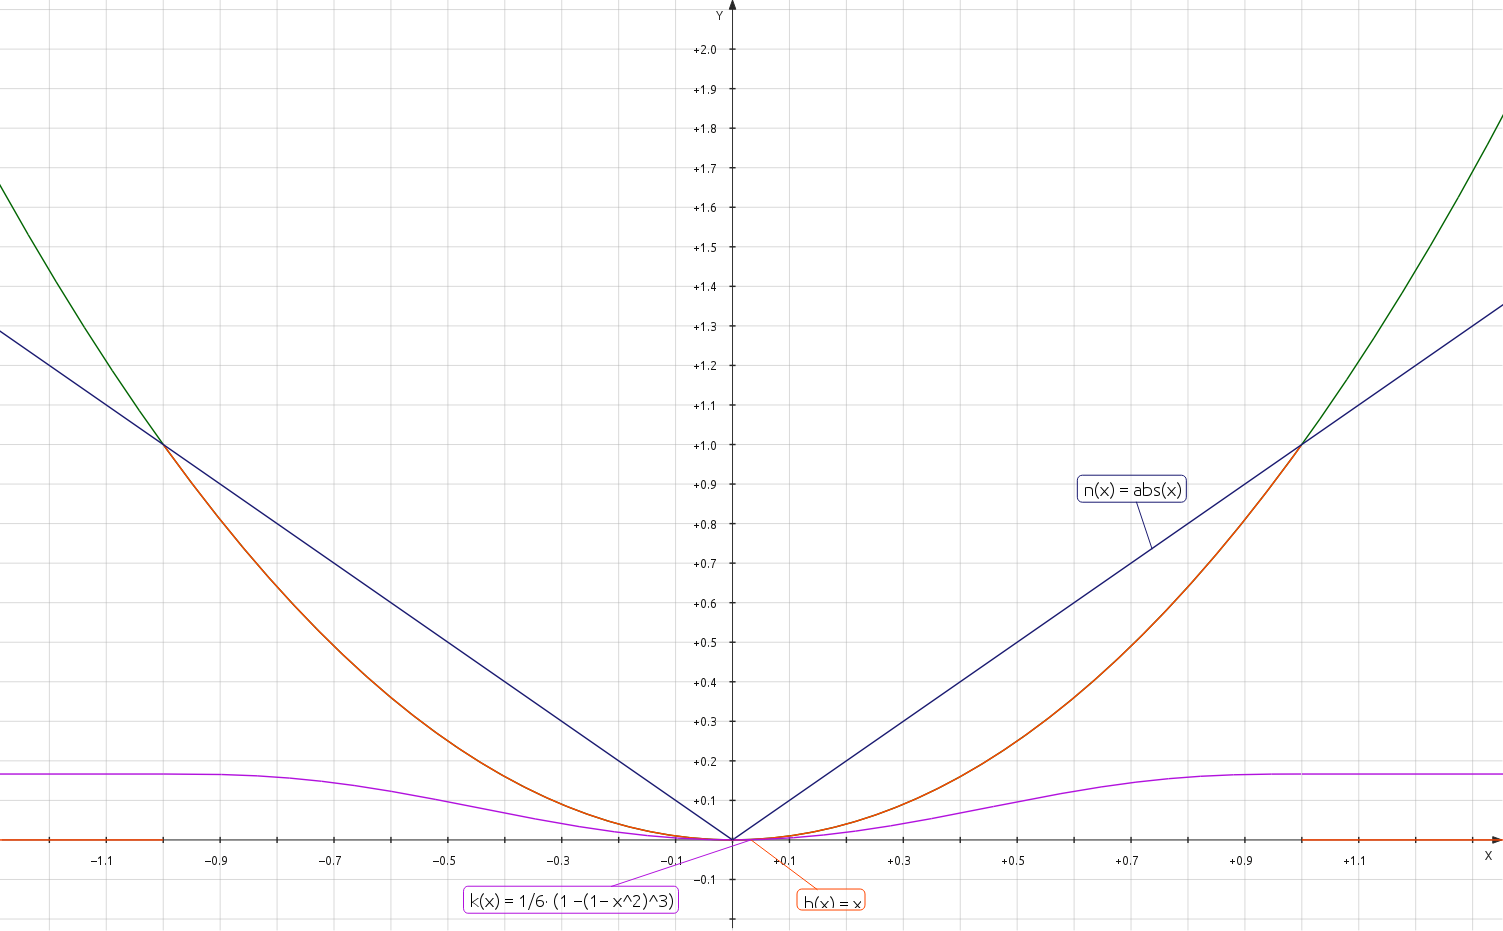
\includegraphics[width=0.7\textwidth]{Chapter4/graphics/objective_functions.png}
	\caption{Exemples de fonctions de coût $\rho$, présentées dans le tableau \ref{tab:ch4_exemple_estimateurs} utilisées par les estimateurs}
	\label{fig:ch4_ml_metrics}
\end{figure}

\begin{figure} 
	\centering
	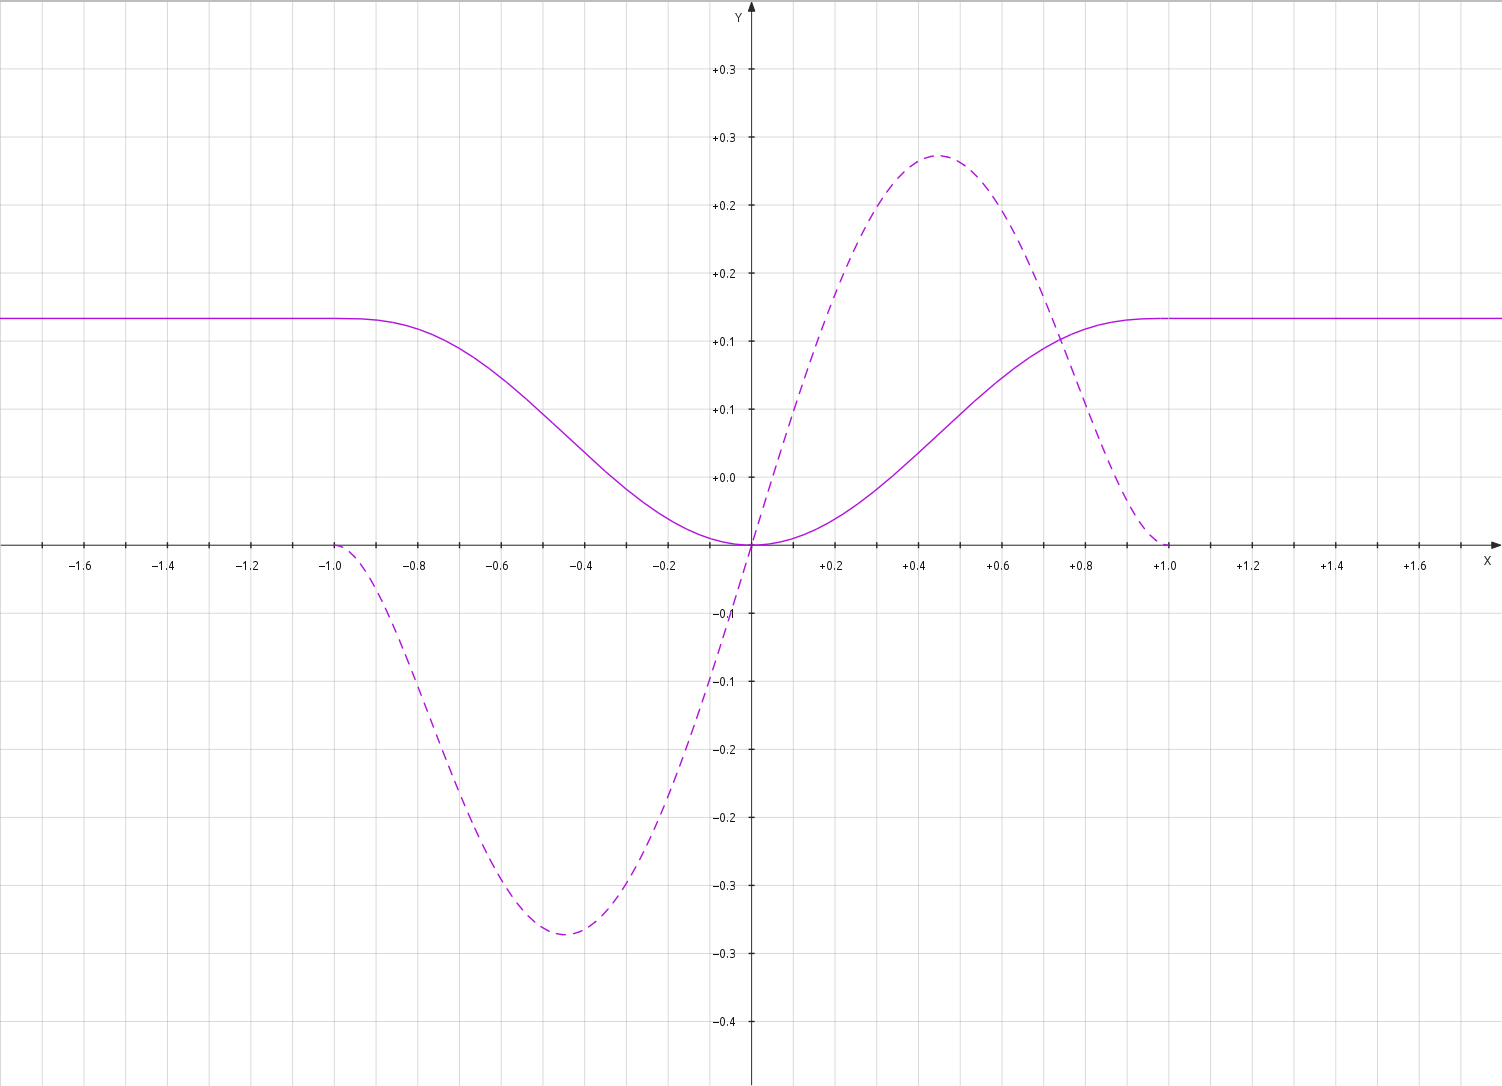
\includegraphics[width=0.5\textwidth]{Chapter4/graphics/tukey_functions.png}
	\caption{Tukey : exemple de fonction de coût $\rho$ (trait plein) et sa dérivée $\Psi$ (pointillés). Les valeurs $\Psi$ = 0 permettent de retrouver les minima locaux de $\rho$}
	\label{fig:ch4_ml_metric_derivatives}
\end{figure}
\clearpage 
